\documentclass[11pt]{article}
\usepackage[margin=1in]{geometry}
\usepackage{volfit_preamble}
\graphicspath{{figures/}}

\title{\textbf{The Wings and the Belly}\\[2pt]
\large SVI as a moment-controlled smile: Lee's bound, the tails it certifies,
and the interior it does not\\[2pt]
\normalsize Vol-Fitter Technical Notes, No.~02 --- lecture edition}
\author{Vol-Fitter}
\date{\today}

% Local symbols for this edition (see the notation ledger, Table 1).
\newcommand{\Iv}{I}                 % working implied volatility sqrt(w/tau)
\newcommand{\wmin}{w_\star}         % minimum total variance
\newcommand{\kmin}{k_\star}         % minimizing log-moneyness
\newcommand{\vmin}{\widetilde v}    % minimum variance handle
\newcommand{\betL}{\beta_L}
\newcommand{\betR}{\beta_R}

\begin{document}
\maketitle
% Auto-generated by gen_svi_moments.py -- do not edit.
\newcommand{\svimommaxerr}{\ensuremath{5.6\times10^{-13}}}
\newcommand{\svimomnfev}{21}
\newcommand{\svimomjwerr}{\ensuremath{3.9\times10^{-16}}}
\newcommand{\svimomgmin}{0.343}
\newcommand{\svimomwingL}{0.1093}
\newcommand{\svimomwingR}{0.0364}
\newcommand{\svimomcountermin}{0.0116}
\newcommand{\svimomcounterlee}{0.174}
\newcommand{\svimomcounterg}{-0.033}
\newcommand{\svimomcounterk}{0.88}
\newcommand{\svimomcountergL}{0.249}
\newcommand{\svimomcountergR}{0.248}
\newcommand{\svimomrigidrms}{147.6}
\newcommand{\svimomrigidmax}{351.9}
\newcommand{\svimomanalyticms}{1.81}
\newcommand{\svimomfdms}{4.15}
\newcommand{\svimomspeedup}{2.29}
\newcommand{\svimomcostdiff}{\ensuremath{2.7\times10^{-33}}}
\newcommand{\svimomhistbefore}{26.3}
\newcommand{\svimomhistafter}{10.2}
\newcommand{\svimomhistspeedup}{2.58}
\newcommand{\svimomhistin}{24.3}
\newcommand{\svimomhistoos}{26.8}
\newcommand{\svimomnodes}{1,576}
\newcommand{\svimomarbold}{20.8}
\newcommand{\svimomarbnew}{9.2}
\newcommand{\svimomlqdarbold}{28.3}
\newcommand{\svimomlqdarbnew}{0.0}
\newcommand{\svimompenalty}{1000}
\newcommand{\svimomleecap}{2.0}
\newcommand{\svimomrawtable}{\begin{tabular}{lr} \toprule Parameter & Value\\ \midrule $a$ & +0.010625\\ $b$ & +0.072887\\ $\rho$ & -0.500000\\ $m$ & +0.058310\\ $s$ & +0.100995\\ \bottomrule \end{tabular}}
\newcommand{\svimomjwtable}{\begin{tabular}{lr} \toprule Handle & Value\\ \midrule $v$ & +0.042500\\ $\psi$ & -0.250000\\ $p$ & +0.750000\\ $c$ & +0.250000\\ $\widetilde v$ & +0.034000\\ \bottomrule \end{tabular}}


\begin{abstract}
A volatility smile answers two questions at once.  Its \emph{wings} report the
tails of the risk-neutral distribution --- how much mass sits far out of the
money --- and Lee's moment formula caps how fast they may grow.  Its
\emph{belly}, the curvature near the money, reports the shape of the centre.
This note reads raw SVI through that division.  SVI draws one expiry's total
implied variance as a tilted hyperbola: strictly convex, linear in both wings,
and unable to turn twice.  We show that its two asymptotic wing slopes
$\betL=b(1-\rho)$ and $\betR=b(1+\rho)$ are exactly the object Lee's bound
constrains, and that the bound lands inside Durrleman's density factor as the
elementary tail limit $g(\pm\infty)=(4-\beta^2)/16$: the wing slope sets the
\emph{sign} of the implied density in the tail, and $\beta\le2$ is precisely the
condition that the tail density stay non-negative.  Every cheap no-arbitrage
guarantee raw SVI can give therefore lives in the wings.  The belly is where it
cannot: a Lee-clean, positive, strictly convex slice (Axel Vogt's classical
counterexample --- minimum variance \svimomcountermin, larger Lee coefficient
\svimomcounterlee, both tails of $g$ at $\approx0.25>0$) still drives $g$ to
\svimomcounterg\ in its interior, so its Black density is negative near
$k\approx\svimomcounterk$.  The jump-wing (SVI-JW) coordinates are the desk's
way of naming this split: two \emph{tail} handles $p,c$ and three \emph{belly}
handles $v,\psi,\vmin$.  We prove the exact regular domain on which the
five handles invert to a raw slice, and show that where they fail to identify
it --- the $\psi=0$ stratum --- what they lose is precisely the belly curvature:
infinitely many raw widths share the same tails and level.  We then fit the
slice the way the split suggests: an unconstrained reparametrization that fences
the tails (the Lee and minimum rows) while the data term fits the belly, with a
closed-form Levenberg--Marquardt Jacobian that recovers a production benchmark
through a JW$\to$raw$\to$fit$\to$JW round trip to \svimommaxerr\ vol bp and runs
\svimomspeedup$\times$ faster than finite differences.  Product status up front:
production fits and stores \emph{raw} SVI and displays model-agnostic ATM
handles; five-handle JW entry, bumping and export are analytical, not shipped.
\end{abstract}

\newpage
\tableofcontents
\newpage

%======================================================================
\section{Two questions a smile answers}
\label{sec:two}

Stand at one expiry and look at the implied-volatility smile as a curve over
log-moneyness.  It is doing two jobs.  Far from the money it is reporting the
\emph{tails} of the risk-neutral law --- the price the market puts on rare
moves --- and near the money it is reporting the \emph{belly}, the local shape
around the forward.  These two jobs are governed by different mathematics.  The
tails obey a hard theorem: Lee's moment formula ties the growth rate of implied
variance in the wings to the number of finite moments of the underlying, and
caps that growth.  The belly obeys no such cheap law; it is where a smile can
look perfectly reasonable and still be arbitrageable.

The organizing claim of this note is that raw SVI wears this division on its
sleeve, and that every guarantee the Vol-Fitter cheaply enforces on an SVI slice
is a \emph{wing} guarantee.  Once that is clear, three otherwise separate facts
become one story: why the coded no-arbitrage screens are tail conditions, why
the classical counterexample that defeats them fails in the \emph{belly}, and
why the trader coordinate system (SVI-JW) is built to separate the two.  We
develop the geometry first, read the tails through Lee's bound, watch the belly
escape, and only then change coordinates and fit.

\paragraph{Conventions and clocks.}
Throughout, $k=\log(K/F_T)$ is log-moneyness against the expiry-$T$ forward
$F_T$, and
\[
w(k)=\text{(Black implied total variance at }k)
\]
is the object SVI models.  The normalized Black price depends only on $k$ and
$w$, so $w$ is recovered from a quoted price without first choosing an
annualization clock.  Vol-Fitter keeps two clocks apart:
\begin{equation}
\Iv_t(k)=\sqrt{\frac{w(k)}{t}},\qquad
\Iv_\tau(k)=\sqrt{\frac{w(k)}{\tau}},
\label{eq:clocks}
\end{equation}
where $t=t_T$ is the plain calendar year fraction and $\tau=\tau_T$ is the
\emph{active variance time} --- calendar time dilated by scheduled events
(Notes~00 and~11), equal to $t$ when the event clock is off.  Production passes
$\tau$ to the calibrator, so unless qualified $\Iv$ means the working quantity
$\Iv_\tau$; changing the clock rescales the annualized number, never $w$.  A
\emph{volatility basis point} (vol bp) is $10^{-4}$ in volatility.  We write the
SVI width as $s$ so that $\sigma$ is free for volatility, and reserve one
differentiation convention: a prime denotes the derivative of a one-variable
function ($w'$, $w''$, $\Iv'$), a subscripted or explicit $\partial$ denotes a
partial ($\partial w/\partial\rho$).

\begin{table}[H]
\centering
\small
\setlength{\tabcolsep}{5pt}
\renewcommand{\arraystretch}{1.18}
\begin{tabular}{@{}lll@{}}
\toprule
Symbol & Meaning & First used\\
\midrule
$k$ & log-moneyness $\log(K/F_T)$ & \eqref{eq:clocks}\\
$w(k)$ & total implied variance (price-derived) & \eqref{eq:raw}\\
$t,\ \tau$ & calendar year fraction; active variance time & \eqref{eq:clocks}\\
$\Iv(k)$ & working implied volatility $\sqrt{w/\tau}$ & \eqref{eq:clocks}\\
$a,b,\rho,m,s$ & raw SVI parameters (width $s$) & \eqref{eq:raw}\\
$\betL,\betR$ & asymptotic wing slopes $b(1\mp\rho)$ of $w$ & \eqref{eq:betas}\\
$\kmin,\ \wmin$ & minimizing $k$; minimum total variance & \eqref{eq:vertex}\\
$g(k)$ & Durrleman density factor & \eqref{eq:g}\\
$v,\psi,p,c,\vmin$ & JW handles: level, ATM slope, wings, floor & \eqref{eq:jwdef}\\
$\chi$ & normalized displacement $m/\sqrt{m^2+s^2}$ & \eqref{eq:chi}\\
$D$ & inverse denominator (an angle gap) & \eqref{eq:D}\\
$\theta$ & unconstrained calibration vector in $\R^5$ & \eqref{eq:reparam}\\
\bottomrule
\end{tabular}
\caption{Notation ledger.  Nothing is reused with a second meaning; the width
is $s$, never $\sigma$, and there is one time symbol per clock.}
\label{tab:ledger}
\end{table}

Raw SVI (Gatheral) postulates that the entire slice is one hyperbola:
\begin{equation}
\boxed{\;w(k)=a+b\Big\{\rho(k-m)+\sqrt{(k-m)^2+s^2}\Big\}.\;}
\label{eq:raw}
\end{equation}
Five parameters, and --- as we are about to see --- exactly two of them, bundled
as $\betL,\betR$, are what Lee's bound touches.  The rest describe the belly.

\begin{invariant}
\begin{enumerate}[leftmargin=1.6em]
\item Every finite $\theta\in\R^5$ maps to a smooth raw hyperbola with $b>0$,
$|\rho|<1$, $s>0$ (\cref{sec:calib}); positivity and no-arbitrage need more.
\item The two coded screens are \emph{tail} conditions: a non-negative floor
$\vmin\ge0$ and Lee's wing cap $\max(\betL,\betR)\le2$.  Both are
finite-weight soft rows, exactly zero on a clean slice, and they bound but do
not certify non-negativity of the Black density in the belly.
\item The raw$\leftrightarrow$JW change of coordinates is exact on the regular
domain of \cref{thm:image}; the singular stratum it omits is a loss of
\emph{belly} information (\cref{rem:psi0}).
\item SVI is one display overlay among several: band, calendar, var-swap, prior
and extrapolation blocks share the series' product targets through
model-specific residuals, and each is byte-identical to its own absence.
\end{enumerate}
\end{invariant}

%======================================================================
\section{One hyperbola with straight wings}
\label{sec:geometry}

Everything below rests on three closed-form facts about \eqref{eq:raw}.  Write
\begin{equation}
x=k-m,\qquad r=\sqrt{x^2+s^2},\qquad q=\sqrt{1-\rho^2}.
\label{eq:short}
\end{equation}

\begin{proposition}[Geometry of one slice]
\label{prop:geom}
Under $b>0$, $|\rho|<1$, $s>0$, the slice $w$ is strictly convex with a single
minimum:
\begin{align}
w'(k)&=b\Big(\rho+\frac{x}{r}\Big), &
w''(k)&=\frac{b\,s^2}{r^3}>0,
\label{eq:deriv}\\
\kmin&=m-\frac{s\rho}{q}, & \wmin&=a+b\,s\,q .
\label{eq:vertex}
\end{align}
Its far field is two straight rays,
\begin{equation}
w(k)=\betL\,|k|+O(1)\ (k\to-\infty),\quad
w(k)=\betR\,k+O(1)\ (k\to+\infty),\quad
\betL=b(1-\rho),\ \betR=b(1+\rho).
\label{eq:betas}
\end{equation}
\end{proposition}

\begin{proof}
Differentiating \eqref{eq:raw} gives \eqref{eq:deriv}; since $b,s>0$, $w''>0$
for every finite $k$, so a stationary point is the unique global minimum.
Solving $w'=0$ gives $x=-s\rho/q$, hence $r=s/q$ and \eqref{eq:vertex}.  In
either wing $r=|x|+o(1)$, which yields \eqref{eq:betas}.
\end{proof}

Two consequences are worth stating plainly, because they drive the rest of the
note.  First, $w''>0$ \emph{everywhere}: raw SVI is one globally convex curve
with one belly and one turn of the slope, from $-\betL$ up to $+\betR$
(\cref{fig:wings}A).  This is the model's rigidity, and \cref{sec:rigidity}
returns to it.  Second --- the point of this section --- the tails collapse to
\emph{two numbers}.  As $|k|$ grows, $w(k)/|k|$ converges to $\betL$ on the put
side and $\betR$ on the call side (\cref{fig:wings}B); no other feature of the
slice survives to infinity.  Whatever the market's tails are worth, SVI records
them in $\betL$ and $\betR$ alone.

\begin{figure}[H]
\centering
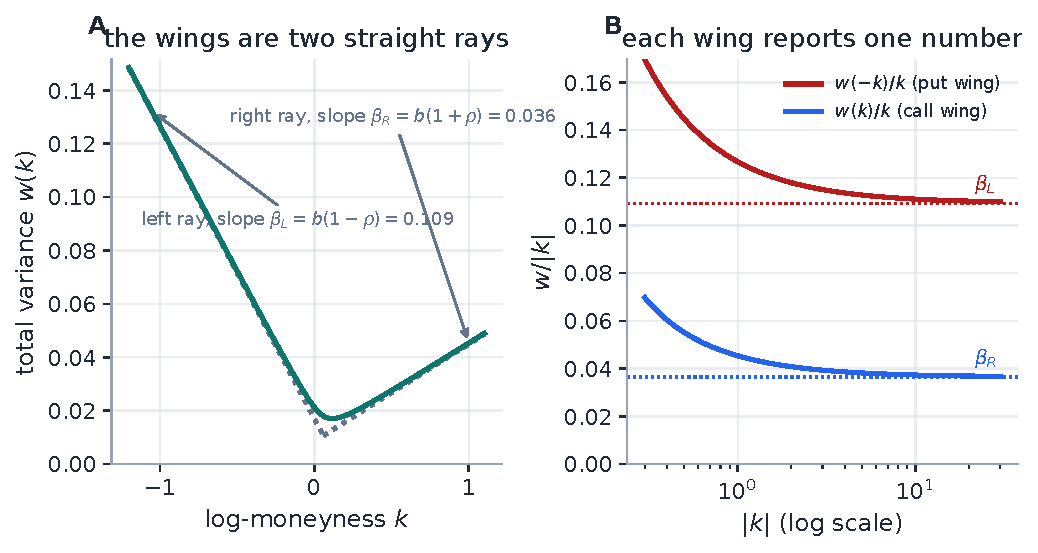
\includegraphics[width=\textwidth]{fig_svimom_wings.pdf}
\caption{The wings are a two-number reading of the tails.  Panel A: the total
variance approaches two straight asymptotes, steeper on the put side for the
equity skew $\rho<0$.  Panel B: $w(k)/|k|$ collapses onto the constants $\betL$
and $\betR$ as $|k|\to\infty$ --- each wing reports exactly one slope, and those
two slopes are all that Lee's bound of \cref{sec:lee} can see.}
\label{fig:wings}
\end{figure}

\begin{heuristic}
Read \eqref{eq:raw} as a rounded hinge.  Far out, the hinge has forgotten its
rounding and shows two straight rays of slope $\betL$ (left) and $\betR$
(right).  Near the centre, $s$ decides how sharply one ray turns into the other,
$m$ sets where the rounding sits, and $a$ raises the whole curve.  The tilt
$\rho$ divides a fixed total steepness $\betL+\betR=2b$ between the two sides.
The wings are tails; the region where $s$ matters is the belly.
\end{heuristic}

%======================================================================
\section{Lee's bound is a statement about the wings}
\label{sec:lee}

Why should a wing slope be capped at all?  Because it is a moment barometer.
Lee's moment formula \cite{Lee2004} says that if the underlying has $\bar p$
finite moments beyond the first, the right-wing implied variance grows no faster
than $\betR\,k$ with a slope controlled by $\bar p$, and symmetrically on the
left; in the limiting case of a distribution on the edge of losing all moments,
the slope reaches $2$.  Heavier tails would demand a steeper wing, and a wing
steeper than $2$ is not the tail of \emph{any} probability distribution.  For a
model whose wings are exactly linear, this is not an asymptotic nicety --- it is
a sharp, checkable inequality on two of its parameters.

The cleanest way to see the bound bite is to follow it inside the object that
actually tests for arbitrage.  A positive, $C^2$ total-variance slice with the
right wing behaviour is free of butterfly arbitrage iff the Black density it
implies is non-negative, and Durrleman \cite{Durrleman2010} writes that density,
up to a strictly positive prefactor, as
\begin{equation}
g(k)=\Big(1-\frac{k\,w'(k)}{2w(k)}\Big)^2
-\frac{w'(k)^2}{4}\Big(\frac{1}{w(k)}+\frac14\Big)+\frac{w''(k)}{2}\ \ge\ 0
\quad\forall k .
\label{eq:g}
\end{equation}
The connection to the wings is a one-line limit.

\begin{proposition}[The wing slope sets the sign of the tail density]
\label{prop:tail}
For a structurally valid positive raw slice,
\begin{equation}
\lim_{k\to-\infty}g(k)=\frac{4-\betL^2}{16},\qquad
\lim_{k\to+\infty}g(k)=\frac{4-\betR^2}{16}.
\label{eq:gtail}
\end{equation}
Hence each tail of the density stays non-negative iff the corresponding wing
slope satisfies $\beta\le2$, and the call-price boundary
$\lim_{k\to+\infty}d_+(k)=-\infty$ (equivalently, the normalized call vanishes
at infinite strike) holds exactly when $\betR<2$.
\end{proposition}

\begin{proof}
In either wing $w\sim\beta|k|$, $|w'|\to\beta$, and $w''\to0$ by
\eqref{eq:deriv}.  The first bracket of \eqref{eq:g} tends to
$1-\tfrac12=\tfrac12$, so its square tends to $\tfrac14$; the middle term tends
to $\beta^2/16$ because $1/w\to0$; the last term vanishes.  This gives
\eqref{eq:gtail}.  For the boundary, with $d_+(k)=-k/\sqrt{w}+\tfrac12\sqrt{w}$
and $w\sim\betR k$ on the right,
\[
d_+(k)=\sqrt{k}\Big(-\tfrac{1}{\sqrt{\betR}}+\tfrac{\sqrt{\betR}}{2}\Big)+o(\sqrt k),
\]
whose leading coefficient is negative exactly for $\betR<2$; at $\betR=2$ the
two terms cancel and $d_+\to0$.
\end{proof}

\Cref{fig:moments} makes the mechanism visible.  The map
$\beta\mapsto(4-\beta^2)/16$ is a downward parabola crossing zero at Lee's cap
$\beta=2$: below the cap the tail of $g$ is a positive constant, above it a
negative one.  Carried into a concrete slice, a wing with $\beta=1.6$ settles
onto a positive plateau far out, while a wing with $\beta=2.3$ settles onto a
negative one --- a butterfly arbitrage that lives arbitrarily deep in the tail.

\begin{figure}[H]
\centering
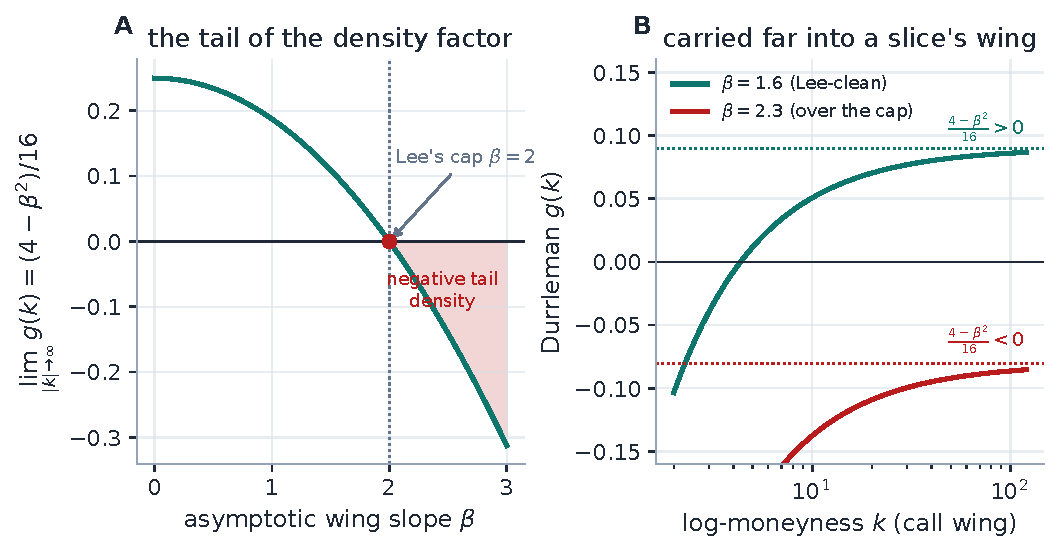
\includegraphics[width=\textwidth]{fig_svimom_moments.pdf}
\caption{Lee's bound, inside the density.  Panel A: the asymptotic value of the
Durrleman factor is $(4-\beta^2)/16$, which changes sign exactly at $\beta=2$;
past the cap the far-tail density is negative.  Panel B: two symmetric slices
differing only in wing slope, followed far out --- $\beta=1.6$ rises to its
positive tail limit, $\beta=2.3$ falls to its negative one.  The wing slope is
not cosmetic; it fixes the sign of the density in the tail.}
\label{fig:moments}
\end{figure}

\begin{proposition}[The coded screens, in JW units]
\label{prop:screensjw}
Under the conversion of \cref{sec:jw}, the two production screens read directly
on the wing handles: the floor condition $\wmin\ge0$ is $\vmin\ge0$, and Lee's
cap $b(1+|\rho|)\le\beta_{\max}$ is
\[
\max(p,c)\,\sqrt{v\tau}\ \le\ \beta_{\max}\ (=\svimomleecap).
\]
\end{proposition}

\begin{proof}
The first is the definition of $\vmin$ (\cref{sec:jw}) times $\tau>0$.  For the
second, $\betL=p\sqrt{w_0}$ and $\betR=c\sqrt{w_0}$ with $w_0=v\tau$
(\cref{sec:jw}), so $b(1+|\rho|)=\max(\betL,\betR)=\max(p,c)\sqrt{v\tau}$.
\end{proof}

So a desk can sanity-check a smile before touching the belly: floor
non-negative, larger wing handle under the cap.  Both are wing statements.  The
belly is a different matter.

\paragraph{Exercise 1.}
Show from \eqref{eq:betas} that $\betL+\betR=2b$ and $\betR-\betL=2b\rho$, so
the two wing slopes carry exactly the same information as $(b,\rho)$.  Deduce
that Lee's cap constrains only the steeper wing, and that a put-skewed slice
($\rho<0$) can violate it on the put side while the call side is far from the
bound.

%======================================================================
\section{The belly escapes}
\label{sec:belly}

The word ``convex'' hides two different second derivatives.  Raw SVI has
$w''>0$ by construction (\cref{prop:geom}).  A butterfly spread, however, tests
the convexity of the option \emph{price} in strike, which is the sign of $g$ in
\eqref{eq:g}, and $g$ mixes $w$, $w'$ and $w''$.  In the wings these agree ---
$g$'s sign is Lee's --- but in the belly they need not.  It is worth fixing four
increasingly strong meanings of ``valid'' once, because the note turns on the
gaps between them.

\begin{table}[H]
\centering
\small
\setlength{\tabcolsep}{5pt}
\begin{tabular}{@{}p{0.19\textwidth}p{0.34\textwidth}p{0.40\textwidth}@{}}
\toprule
Tier & Mathematical statement & Production status\\
\midrule
Structural & $b>0$, $|\rho|<1$, $s>0$ & hard, by reparametrization
(\cref{sec:calib})\\
Tail-clean & $\wmin\ge0$ and $\max(\betL,\betR)\le2$ & the two soft coded
screens; zero on a clean slice\\
Butterfly-clean & $g(k)\ge0$ for all $k$ (with the call boundary) & measured,
not certified by the two screens\\
Calendar-clean & $w_{T_1}(k)\le w_{T_2}(k)$ for $T_1<T_2$ & soft
model-agnostic hinge (Note~10); not structural\\
\bottomrule
\end{tabular}
\caption{Four tiers of ``valid.''  The first is hard, the second soft and
confined to the tails, and the last two require conditions no single raw
coefficient box supplies.  The counterexample below sits in the gap between
tiers two and three: tail-clean, butterfly-dirty.}
\label{tab:tiers}
\end{table}

That the tail screens do not reach tier three is not a worry in the abstract ---
it is a specific, classical slice.  Axel Vogt's example, reproduced as
Example~3.1 by Gatheral and Jacquier \cite{GatheralJacquier2014}, is
\[
(a,b,\rho,m,s)=(-0.0410,\ 0.1331,\ 0.3060,\ 0.3586,\ 0.4153).
\]
Its minimum total variance is \svimomcountermin\ (floor clean), its larger Lee
coefficient is \svimomcounterlee\ (far under the cap of \svimomleecap), and by
\eqref{eq:gtail} \emph{both} tails of $g$ sit at $\approx0.25>0$: the slice is
impeccable in the wings.  Yet $g$ dips to \svimomcounterg\ near
$k\approx\svimomcounterk$ --- in the belly, between the two clean tails --- so
the Black density is negative there and the slice is genuinely arbitrageable
(\cref{fig:belly}).  Strict convexity of $w$ did not protect strike-convexity of
the price.

\begin{figure}[H]
\centering
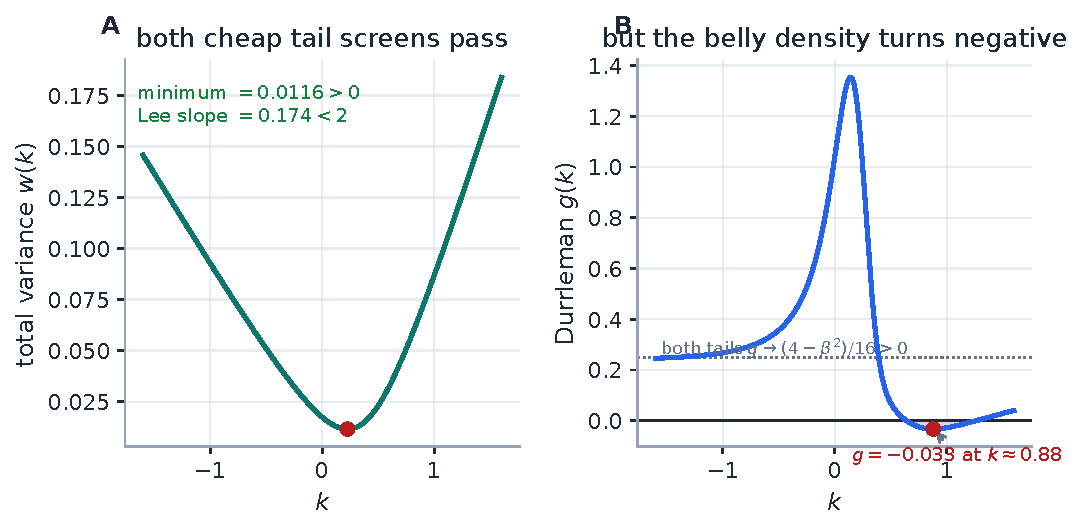
\includegraphics[width=\textwidth]{fig_svimom_belly.pdf}
\caption{The honesty centrepiece.  Panel A: Axel Vogt's slice is positive,
strictly convex, with a positive minimum and a Lee slope far under the cap ---
both cheap tail screens pass.  Panel B: its Durrleman factor approaches the
positive tail limits $(4-\beta^2)/16$ on both sides (dotted), yet turns negative
in the belly.  The screens fence the tails; the interior escapes them.}
\label{fig:belly}
\end{figure}

The exact butterfly-free domain of raw SVI is known --- Martini and Mingone
\cite{MartiniMingone2022} characterize it completely --- but it is not one short
inequality: the test involves parameter rescaling, root finding and a numerical
minimization.  Vol-Fitter's calibrator does not implement that certified domain.
It instead \emph{bounds, measures, and optionally repairs} in a stack of four
layers, at increasing distance from the core fit:
\begin{enumerate}[leftmargin=1.6em]
\item \textbf{Core screens} (always in the objective): the floor and Lee rows of
\cref{eq:penalties}, finite-weight, zero on a tail-clean slice.
\item \textbf{Extrapolated-region enforcement} (opt-in, default off; Notes
09--10): tapered rows penalizing sampled $g<0$ on the slice's own envelope, a
tapered calendar hinge against the previous displayed slice, and a wing-order
hinge.  Only this small block is finite-differenced, so the fit runs a hybrid
Jacobian.
\item \textbf{Advisory diagnostics} (always on): the Quality view measures and
reports the remaining extrapolated-region $g<0$ per fit --- measurement, not
enforcement.
\item \textbf{Publish-time wing projection} (export only; Note~09): a discrete
projection of the exported wing samples that raises prices only, leaving the
fitted core pinned.
\end{enumerate}
None of these turns a fitted SVI slice into a certified butterfly-free object;
together they bound the tails, measure the belly, and clean the boundary where
extrapolation matters.

\paragraph{How $g$ is measured is part of the guarantee.}
An earlier backtest metric evaluated $g$ by finite-differencing
\emph{reconstructed option prices}, and its numerical noise flagged
\svimomlqdarbold\% of provably-clean LQD slices as arbitrageable.  Recomputed
analytically from each model's own $(w,w',w'')$, the LQD rate reads
\svimomlqdarbnew\%, and SVI's flagged rate fell from \svimomarbold\% to
\svimomarbnew\% --- the survivors being genuine belly violations of the kind in
\cref{fig:belly}.  The production rule that came out of that audit: the
diagnostic is always computed on model derivatives, never by differencing
prices (Note~09 gives the cross-model treatment).  It is a reminder that a
badly \emph{measured} $g$ can manufacture arbitrage that isn't there, just as a
tail-only screen can miss arbitrage that is.

\subsection{The two soft screens, precisely}
\label{sec:penalties}

The optimizer adds to the data residual two rows that are exactly zero on a
tail-clean slice and grow linearly past the boundary:
\begin{equation}
r_{\mathrm{core}}(\theta)=W\begin{pmatrix}
\max\!\big(-(a+b\,s\,q),\ 0\big)\\[2pt]
\max\!\big(b(1+|\rho|)-\beta_{\max},\ 0\big)
\end{pmatrix},\qquad q=\sqrt{1-\rho^2},
\label{eq:penalties}
\end{equation}
with residual multiplier $W=\svimompenalty$ and cap $\beta_{\max}=\svimomleecap$.
The first forbids negative total variance at the belly's floor; the second is
Lee's wing bound.  Because both vanish on a clean fit, a tail-clean smile is
byte-identical with or without them: they are a feasibility fence, not a
regularizer.

\begin{caution}
Read $W$ for what it is.  It multiplies the \emph{residual} rows, so the
least-squares objective receives an effective $W^2$ on the squared violation;
and the two rows do not even share a unit --- one is a total variance, the other
a dimensionless slope --- so $W$ is a residual multiplier, not a ``weight in
vol$^2$.''  It is deliberately large enough to dominate a violated constraint
and invisible on a clean one.  It is not a fit-quality dial: raising it cannot
improve a feasible fit, and lowering it only lets the optimizer wander into the
arbitrageable cone.  Both fences are also adjustable rather than unconditional
--- the weight can be set to zero, or the cap raised above $2$ --- so they are
configuration, not guarantees.
\end{caution}

%======================================================================
\section{Trader coordinates that split tail from belly}
\label{sec:jw}

Raw $(a,b,\rho,m,s)$ are excellent computational coordinates and poor market
language: no single one is ``the level'' or ``the skew,'' and, as
\cref{fig:entangle} shows, three of them move a tail and the belly at once.  A
desk wants to name the smile by its features: where ATM volatility sits, how
steeply it leaves the money, how heavy each wing is, and where it bottoms.  The
jump-wing parametrization does exactly this, and --- the reading this note
presses --- it sorts the five numbers into \emph{two tail handles and three
belly handles}.

\begin{figure}[H]
\centering
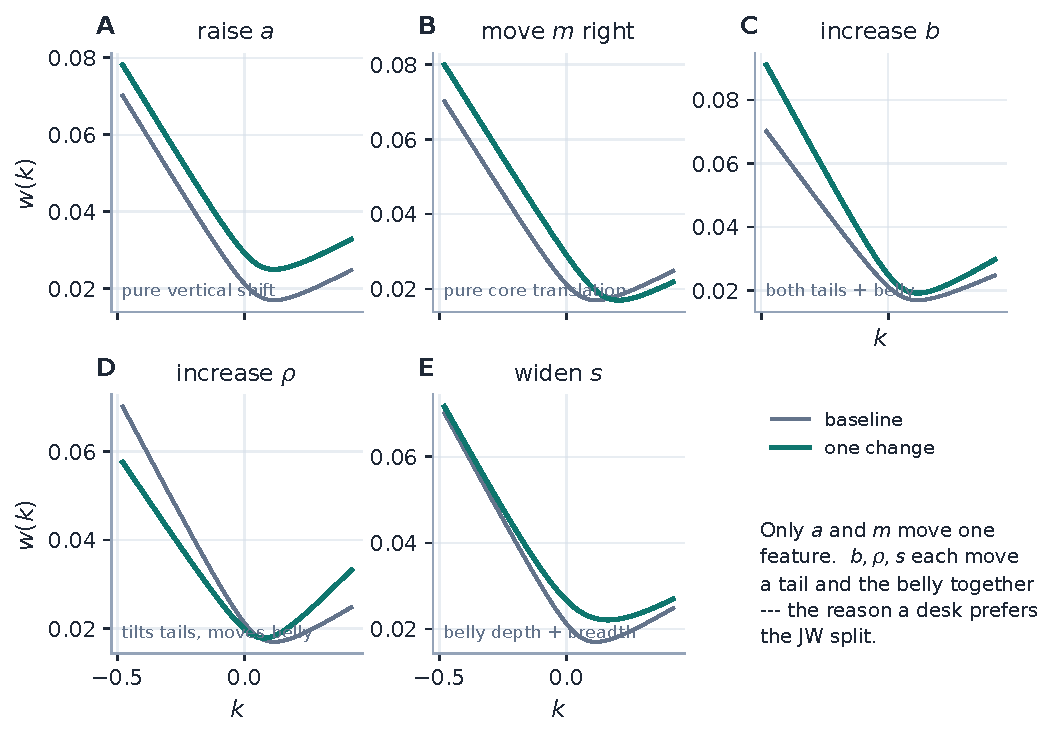
\includegraphics[width=0.98\textwidth]{fig_svimom_entangle.pdf}
\caption{Why raw coordinates are poor market language.  Only $a$ (vertical
shift) and $m$ (core translation) move a single feature.  Each of $b,\rho,s$
moves a wing \emph{and} the belly together, so a trader cannot dial one market
observable without disturbing others --- the motivation for a second chart.}
\label{fig:entangle}
\end{figure}

\begin{definition}[SVI-JW handles]
\label{def:jw}
At variance clock $\tau$, with $w_0=w(0)$ and $\wmin=\min_k w$, the jump-wing
coordinates of a slice are
\begin{equation}
\underbrace{v=\frac{w_0}{\tau},\quad
\psi=\big(\sqrt{w}\big)'(0),\quad
\vmin=\frac{\wmin}{\tau}}_{\text{belly handles}},\qquad
\underbrace{p=\frac{\betL}{\sqrt{w_0}},\quad
c=\frac{\betR}{\sqrt{w_0}}}_{\text{tail handles}} .
\label{eq:jwdef}
\end{equation}
\end{definition}

Substituting \eqref{eq:raw} gives the classical closed forms
\cite[Sec.~3.3]{GatheralJacquier2014}:
\begin{equation}
v=\frac{w_0}{\tau},\quad
\psi=\frac{b}{2\sqrt{w_0}}\Big(\rho-\frac{m}{\sqrt{m^2+s^2}}\Big),\quad
p=\frac{b(1-\rho)}{\sqrt{w_0}},\quad
c=\frac{b(1+\rho)}{\sqrt{w_0}},\quad
\vmin=\frac{a+b\,s\,q}{\tau}.
\label{eq:rawtojw}
\end{equation}
The split is not cosmetic.  The three belly handles are read on the
implied-volatility chart, and the two tail handles are read on the
total-variance chart, in different units:
\begin{equation}
\Iv(0)=\sqrt v,\quad
\Iv'(0)=\frac{\psi}{\sqrt\tau},\quad
\Iv(\kmin)=\sqrt{\vmin},\qquad
\betL=p\sqrt{v\tau},\quad
\betR=c\sqrt{v\tau}.
\label{eq:jwunits}
\end{equation}
Thus $v,\vmin$ are \emph{variances} (the IV chart shows their square roots);
$\psi$ is the ATM slope of \emph{total volatility} $\sqrt w$, equal to $\sqrt\tau$
times the working-IV slope, \emph{not} the plotted tangent; and $p,c$ are
normalized \emph{total-variance} wing slopes, not slopes of the IV curve.
\Cref{fig:handles} annotates a fitted slice in exactly these units, with the
tail handles on the total-variance panel where they live.

\begin{figure}[H]
\centering
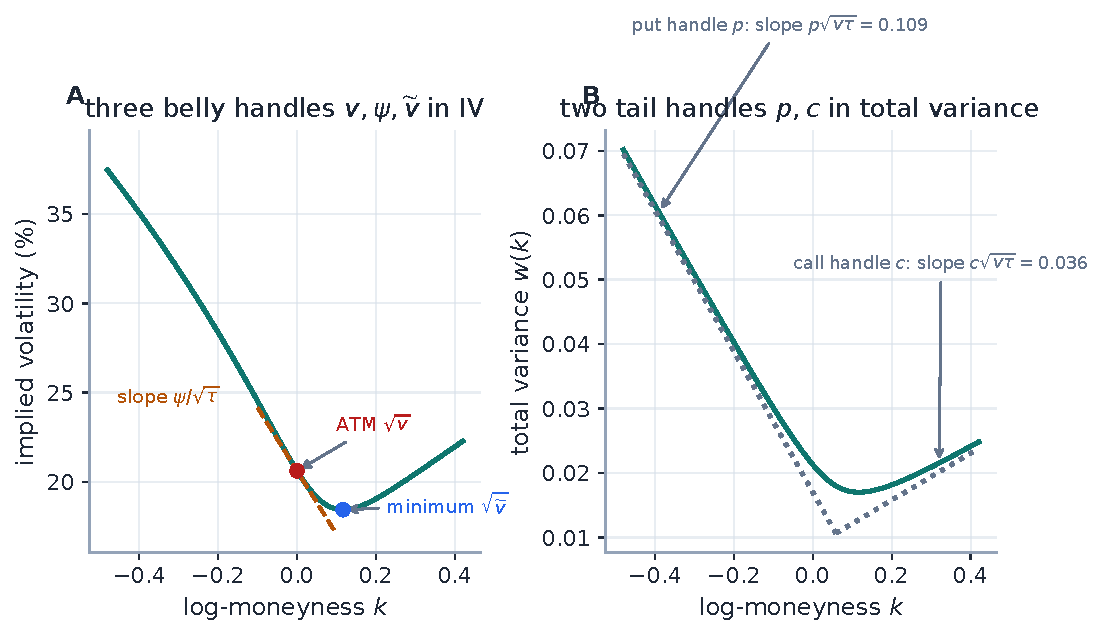
\includegraphics[width=\textwidth]{fig_svimom_handles.pdf}
\caption{The five handles in their honest units.  Panel A (IV): the three belly
handles --- the level $\sqrt v$, the minimum $\sqrt{\vmin}$, and the ATM tangent
of slope $\psi/\sqrt\tau$.  Panel B (total variance): the two tail handles, the
asymptote slopes $p\sqrt{v\tau}$ and $c\sqrt{v\tau}$.  Plotting all five on one
IV axis would give the wing handles units they do not have.}
\label{fig:handles}
\end{figure}

\begin{table}[H]
\centering
\small
\setlength{\tabcolsep}{5pt}
\begin{tabular}{@{}p{0.07\textwidth}p{0.10\textwidth}p{0.23\textwidth}p{0.28\textwidth}p{0.18\textwidth}@{}}
\toprule
Handle & Reads & Functional & Visible as & Common mistake\\
\midrule
$v$ & belly & $w(0)/\tau$ & ATM IV is $\sqrt v$ & treating $v$ as a volatility\\
$\psi$ & belly & $(\sqrt w)'(0)$ & IV tangent is $\psi/\sqrt\tau$ & calling $\psi$ the plotted slope\\
$\vmin$ & belly & $\wmin/\tau$ & minimum IV is $\sqrt{\vmin}$ & assuming positivity from the name\\
$p$ & tail & $\betL/\sqrt{w_0}$ & put slope $p\sqrt{v\tau}$ & reading it on the IV axis\\
$c$ & tail & $\betR/\sqrt{w_0}$ & call slope $c\sqrt{v\tau}$ & reading it on the IV axis\\
\bottomrule
\end{tabular}
\caption{Three belly handles and two tail handles, in three related but distinct
languages: annualized variance, total-volatility skew, and normalized
total-variance wings.  Keeping the units explicit prevents nearly every JW
misreading.}
\label{tab:handles}
\end{table}

\subsection{Inverting the handles, and where the belly information is lost}
\label{sec:inverse}

Reading JW from raw is evaluation.  The reverse --- reconstructing a whole
hyperbola from five measurements --- is the interesting direction, and it is the
one the shipped converter \texttt{jw\_to\_raw} computes (today its only
repository caller is a benchmark test; see the product-status note below).  The
two tail handles fix the scale and tilt,
\begin{equation}
b=\frac{\sqrt{w_0}}{2}(p+c),\qquad \rho=\frac{c-p}{c+p},\qquad w_0=v\tau,
\label{eq:invwings}
\end{equation}
the ATM slope fixes the normalized displacement
\begin{equation}
\chi:=\frac{m}{\sqrt{m^2+s^2}}=\rho-\frac{4\psi}{p+c},
\label{eq:chi}
\end{equation}
and the belly gap $v-\vmin$ then sets the width.  Writing
\begin{equation}
D(\rho,\chi)=\frac{1-\rho\chi}{\sqrt{1-\chi^2}}-\sqrt{1-\rho^2},
\label{eq:D}
\end{equation}
the remaining coordinates are
\begin{equation}
s=\frac{(v-\vmin)\,\tau}{b\,D(\rho,\chi)},\qquad
m=\frac{\chi\,s}{\sqrt{1-\chi^2}},\qquad
a=\vmin\tau-b\,s\sqrt{1-\rho^2},
\label{eq:inverse}
\end{equation}
because $\sqrt{m^2+s^2}=s/\sqrt{1-\chi^2}$, so subtracting $\wmin=\vmin\tau$ from
$w_0=v\tau$ leaves $b\,s\,D$.  The denominator $D$ has a clean geometric form:
setting $\rho=\sin\alpha$, $\chi=\sin\gamma$,
\begin{equation}
D=\frac{1-\cos(\alpha-\gamma)}{\cos\gamma}\ \ge\ 0,
\label{eq:Dangle}
\end{equation}
with equality iff $\chi=\rho$.  This single observation gives both the domain
and the singularity.

\begin{theorem}[The full smooth image of the JW map]
\label{thm:image}
Fix $\tau>0$ and restrict raw SVI to $b>0$, $|\rho|<1$, $s>0$, $w_0>0$.
\begin{enumerate}[leftmargin=1.6em]
\item A JW point has a unique regular inverse iff
\begin{equation}
v>0,\quad p>0,\ c>0,\quad -\frac p2<\psi<\frac c2,\quad \psi\ne0,\quad \vmin<v,
\label{eq:regdom}
\end{equation}
and then \eqref{eq:invwings}--\eqref{eq:inverse} return it.
\item The image also contains the singular stratum
$v>0,\ p,c>0,\ \psi=0,\ \vmin=v$, every point of which is represented by
\emph{infinitely many} raw slices.  There are no other smooth, nondegenerate
image points.
\end{enumerate}
\end{theorem}

\begin{proof}
If $p,c>0$ then \eqref{eq:invwings} gives $b>0$ and $\rho\in(-1,1)$; conversely
a valid slice has $p,c>0$.  From \eqref{eq:chi}, using $(\rho-1)(p+c)=-2p$ and
$(\rho+1)(p+c)=2c$,
\[
|\chi|<1\iff \rho-1<\tfrac{4\psi}{p+c}<\rho+1\iff -\tfrac p2<\psi<\tfrac c2,
\]
which keeps $m=\chi s/\sqrt{1-\chi^2}$ finite.  By \eqref{eq:Dangle}, $D>0$
exactly when $\chi\ne\rho$, i.e.\ $\psi\ne0$; then $s>0$ in \eqref{eq:inverse}
requires the numerator $v-\vmin>0$.  Each failure breaks a requirement: $p+c\le0$
or one of $p,c\le0$ forces $b\le0$ or $|\rho|\ge1$; $\psi$ outside the band sends
$|\chi|\ge1$; $\psi=0$ zeroes $D$; $\vmin\ge v$ makes $s\le0$.  For the singular
stratum, $\psi=0$ gives $\chi=\rho$, i.e.\ $\kmin=0$ by \eqref{eq:vertex}, so ATM
\emph{is} the minimum and $\vmin=v$.  Conversely, fix $v,p,c$ on the stratum;
\eqref{eq:invwings} sets $b,\rho$, and for \emph{any} $s>0$,
$m=\rho s/\sqrt{1-\rho^2}$ with $a=v\tau-b\,s\sqrt{1-\rho^2}$ yields $\kmin=0$,
$\wmin=w_0=v\tau$, and reproduces the same five handles.
\end{proof}

\begin{remark}[The blind spot is the belly]
\label{rem:psi0}
The free width $s$ on the singular stratum is not an abstract degeneracy: it is
exactly the belly curvature.  On that stratum ATM sits at the minimum, and the
handles pin the level $v$ and both tails $p,c$ but say nothing about how sharply
the curve turns through its bottom.  \Cref{fig:singular}B shows three raw bodies
that agree on $(v,0,p,c,v)$ and differ only in how rounded the belly is.  The
jump-wing chart is a fine coordinate system \emph{away} from this stratum and
ill-conditioned near it: by \eqref{eq:Dangle} the denominator vanishes
\emph{quadratically},
\begin{equation}
D\sim\frac{(\chi-\rho)^2}{2(1-\rho^2)^{3/2}}=\frac{8\psi^2}{(p+c)^2(1-\rho^2)^{3/2}},
\qquad \psi\to0,
\label{eq:Dasym}
\end{equation}
so recovering a finite width as $\psi\to0$ forces $v-\vmin=O(\psi^2)$, and a naive
evaluation of \eqref{eq:D} subtracts two nearly equal numbers.  The reference
implementation of \cref{app:ref} uses an algebraically identical but
cancellation-free denominator; no rearrangement can restore a curvature the
handles never carried.
\end{remark}

\begin{figure}[H]
\centering
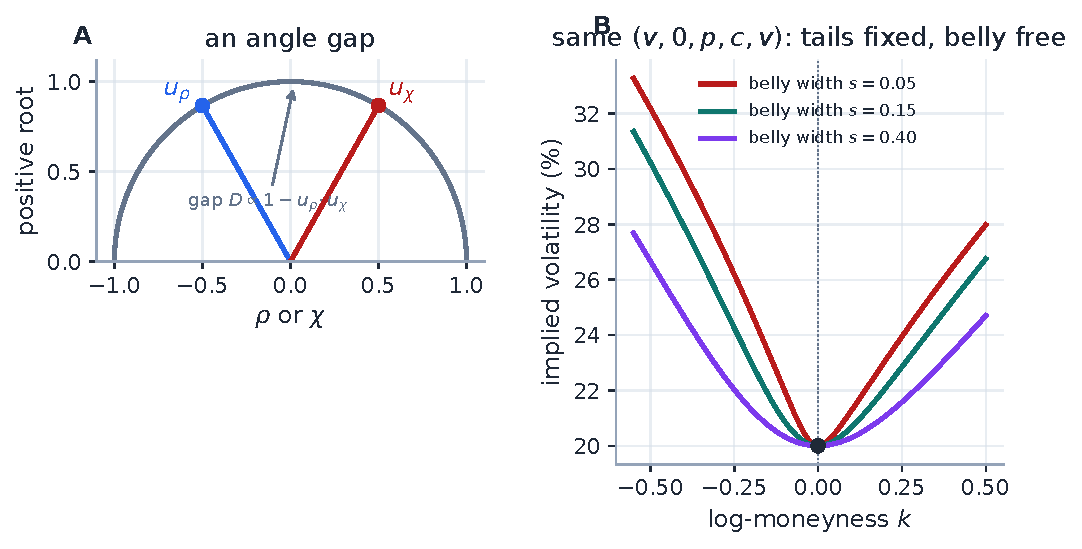
\includegraphics[width=\textwidth]{fig_svimom_singular.pdf}
\caption{The $\psi=0$ stratum is a belly blind spot.  Panel A: the inverse
denominator $D$ is an angular gap between the unit vectors $u_\rho$ and $u_\chi$;
it closes exactly when $\psi=0$.  Panel B: three raw slices with identical
$(v,0,p,c,v)$ --- same level, same asymptotic rays --- differing only in belly
width $s$.  The handles fix the tails and lose the interior curvature.}
\label{fig:singular}
\end{figure}

\begin{caution}[title={Caution --- product status, and the unguarded converter}]
Production calibration fits and stores \emph{raw} SVI as the selected overlay
family and displays three model-agnostic numeric handles --- ATM vol, skew and
curvature by finite differences of the displayed curve --- for every model.
There is no backend \texttt{raw\_to\_jw}, no five-handle JW API/UI entry, no JW
bumping and no JW export; those are candidate features, not shipped ones.  The
shipped \texttt{jw\_to\_raw} implements \eqref{eq:invwings}--\eqref{eq:inverse}
with \emph{zero} domain checks, and its failure modes differ by case rather than
being uniformly silent: a scalar $p+c=0$ raises a division error; $\psi$ outside
$(-p/2,c/2)$ takes the square root of a negative and returns NaNs; $\vmin\ge v$
returns $s\le0$, not a slice; a near-zero $\psi$ amplifies rounding.  This is
deliberate --- the only caller feeds it benchmark handles well inside
\cref{thm:image} --- but it makes the regular domain a \emph{contract}, now
test-locked.  Any future user-facing JW workflow must validate \eqref{eq:regdom}
first, treat the singular stratum separately, and use the stable denominator.
\end{caution}

\paragraph{Exercise 2.}
On the singular stratum, differentiate the five functionals \eqref{eq:rawtojw}
with respect to $s$ at fixed $(v,\psi,p,c,\vmin)$ using
$m=\rho s/\sqrt{1-\rho^2}$, $a=v\tau-b\,s\sqrt{1-\rho^2}$, and verify that
$\partial(v,\psi,p,c,\vmin)/\partial s=0$.  Conclude that the Jacobian of the
raw$\to$JW map drops rank there --- an analytic statement of the belly blind
spot.

%======================================================================
\section{Fitting the slice: fit the belly, fence the tails}
\label{sec:calib}

The optimizer never handles a bounded raw vector.  It receives $\theta\in\R^5$
and maps
\begin{equation}
a=\theta_1,\quad
b=\operatorname{softplus}(\theta_2),\quad
\rho=\tanh(\theta_3),\quad
m=\theta_4,\quad
s=e^{\theta_5},
\label{eq:reparam}
\end{equation}
so that every finite $\theta$ is a structurally valid hyperbola (tier one of
\cref{tab:tiers}).  This removes the box constraints entirely: the unconstrained
Levenberg--Marquardt (LM) solver never wastes a step on the boundary and never
proposes a nonsensical hyperbola.  It guarantees no more than structure --- $a$
stays free, so a trial slice can still carry negative total variance somewhere,
which the residual handles by flooring $w$ at $10^{-12}$ inside the square root
(a solver device; \texttt{RawSVI.implied\_vol} itself has no floor).  Tail
feasibility is the business of the soft rows \eqref{eq:penalties}; belly
feasibility is not enforced at all, by design.

\paragraph{Objective, weights, start.}
The data term is a plain implied-volatility residual
$r_i=\sqrt{\omega_i}\,(\Iv(k_i)-\Iv_i)$; bid--ask and haircut modes replace it
by a vol-space band hinge with a small mid anchor.  The surfaced quote-weight
choices are \texttt{equal} and \texttt{tv\_density} (Note~07), the same two
every model gets; the low-level API also accepts arbitrary $\omega_i$ (e.g.\
vega$^2$, used by research scripts), which is a code capability, not a setting.
The initializer is geometric and reads the belly and the wings directly: the
argmin of the quoted $w$ seeds $(a,m)$, and two finite-span wing slopes seed
$(b,\rho)$ through \eqref{eq:betas}, after which \eqref{eq:reparam} is inverted
for $\theta_0$.  On a liquid smile a single LM pass converges.

\subsection{The analytic Jacobian, in three layers}
\label{sec:jacobian}

The residual Jacobian is worth deriving, because it is what makes SVI the speed
peer of the other models.  It is three chain-rule layers.  First, the
raw-parameter partials of the hyperbola, with $x,r$ from \eqref{eq:short}:
\begin{equation}
\frac{\partial w}{\partial a}=1,\quad
\frac{\partial w}{\partial b}=\rho x+r,\quad
\frac{\partial w}{\partial\rho}=b\,x,\quad
\frac{\partial w}{\partial m}=-b\Big(\rho+\frac{x}{r}\Big),\quad
\frac{\partial w}{\partial s}=\frac{b\,s}{r}.
\label{eq:partials}
\end{equation}
Second, the data rows live in IV, so the Black chain rule for $\Iv=\sqrt{w/\tau}$:
\begin{equation}
\frac{\partial\Iv}{\partial w}=\frac{1}{2\sqrt{w\tau}}=\frac{1}{2\tau\Iv},
\label{eq:ivchain}
\end{equation}
zeroed wherever the $w\le10^{-12}$ floor is active.  Third, the reparametrization
\eqref{eq:reparam}:
\begin{equation}
\frac{\dd b}{\dd\theta_2}=\operatorname{sigmoid}(\theta_2)=1-e^{-b},\qquad
\frac{\dd\rho}{\dd\theta_3}=1-\rho^2,\qquad
\frac{\dd s}{\dd\theta_5}=s.
\label{eq:reparamchain}
\end{equation}
The hinge rows follow the subgradient convention ``active linear part, else
zero'': the floor row differentiates $-(a+b\,s\,q)$, the Lee row differentiates
$b(1+|\rho|)$ with the $\sgn(\rho)$ subgradient (zero at $\rho=0$), and each is a
zero row where its violation is not strictly positive.  The calibrator uses this
closed form whenever no var-swap or prior block is present; those blocks are not
differentiated and revert the fit to finite differences, exactly as in LQD.
Under extrapolation enforcement the fit is \emph{hybrid}: the rows above stay
analytic and only the small extrapolation block is finite-differenced.

\begin{perfbox}
The solver is Levenberg--Marquardt, not trust-region reflective: on noisy real
chains LM crosses the penalty kinks in far fewer iterations at matched tolerance
(\texttt{trf} at $10^{-10}$ was measured slower on real nodes), so the analytic
Jacobian is a same-convergence drop-in that swaps scipy's $1+P$ finite-difference
evaluations ($P=5$) for one closed-form call.  Two measurements, labelled for
what they are.  (i) This note's private residual/Jacobian microbenchmark on the
25-quote synthetic case (\cref{sec:example}), warmed median of five,
single-threaded on the development machine, core rows only: \svimomfdms\,ms
$\to$ \svimomanalyticms\,ms, a \svimomspeedup$\times$ speed-up with the two
objective costs agreeing to \svimomcostdiff\ (same solution within fit
precision, not bit-identical).  (ii) A historical real-node result: spike-regime
backtest nodes, June-2026 harness, same optimizer and tolerances,
\svimomhistbefore\,ms $\to$ \svimomhistafter\,ms per fit
($\approx\svimomhistspeedup\times$) --- the finding that motivated shipping it.
See \cref{app:perf}.
\end{perfbox}

\begin{figure}[H]
\centering
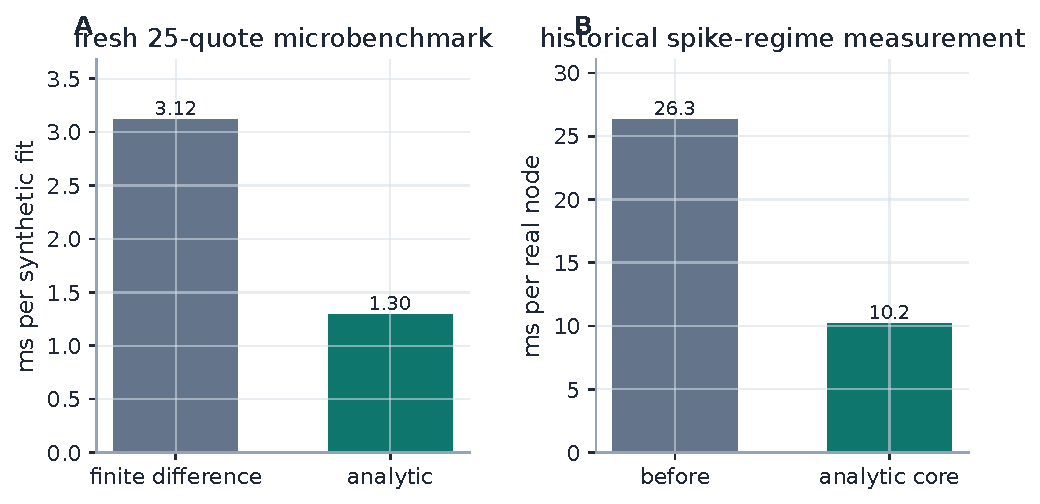
\includegraphics[width=\textwidth]{fig_svimom_timing.pdf}
\caption{The saving is fewer residual evaluations, not a different optimizer.
Panel A is the fresh synthetic microbenchmark; Panel B the historical real-node
measurement.  The two have different scales and provenance and isolate the same
implementation change; machine-dependent numbers and protocol live in
\cref{app:perf}.}
\label{fig:timing}
\end{figure}

\subsection{The optional blocks}
The optional blocks share the series' product targets through model-specific
residuals, and each is byte-identical to its own absence:
\begin{itemize}[leftmargin=1.4em]
\item \textbf{Band fit} (Note~07): the mid residual becomes a vol-space band
hinge with a small mid anchor.
\item \textbf{Calendar hinge} (Note~10): the model-agnostic
$\sqrt{W_{\mathrm{cal}}}\,\max(\text{floor}-w(k),0)$ against the nearer expiry
--- the same target LQD expresses through its quantile, written here on $w$.  A
finite-weight hinge drives crossings down, not provably to zero.
\item \textbf{Extrapolation fences} (default off; Notes 09--10): the tapered
rows of \cref{sec:belly}, hybrid-Jacobian when on.
\item \textbf{Var-swap target} (Note~08) and \textbf{prior persistence}
(Note~13): the same targets as LQD through SVI-native residuals, so the SVI
overlay now receives the prior treatment the primary model does --- closing an
old asymmetry in which SVI overlays got no prior at all.
\end{itemize}

%======================================================================
\section{Worked example: a laboratory round trip}
\label{sec:example}

An exact-family, noise-free recovery is not market evidence; it is the right
laboratory test for a coordinate conversion and a Jacobian, since any visible
miss is an implementation error.  Take $\tau=0.5$ and the jump-wing handles
$(v,\psi,p,c,\vmin)=(0.0425,-0.25,0.75,0.25,0.034)$.  The \emph{production}
\texttt{jw\_to\_raw} builds the target raw slice
$(a,b,\rho,m,s)\approx(0.010625,0.07289,-0.5,0.05831,0.10100)$; we sample 25
noise-free quotes on $[-0.35,0.30]$, refit production raw SVI from the geometric
start, and read the handles back --- a genuine JW$\to$raw$\to$fit$\to$JW loop
whose forward leg is shipped code.

Report two errors, and keep them separate.  The \emph{quote} error --- the
report-space miss --- is a maximum of \svimommaxerr\ vol bp over the 25 quotes,
in \svimomnfev\ residual evaluations.  The \emph{latent} error --- the miss in
the object we actually recovered --- is a maximum jump-wing round-trip deviation
of \svimomjwerr\ across all five handles (\cref{tab:jwcase} reproduces the
target to display precision).  The recovered wing slopes are $\betL=\svimomwingL$
(put) and $\betR=\svimomwingR$ (call).  Both errors are at machine precision
because the target \emph{is} an SVI slice: the exercise validates the optimizer
and the exact conversion, and says nothing about SVI's expressiveness on a
non-SVI market.  On the diagnostic grid $g$ stays above \svimomgmin\
(\cref{fig:recovery}C).

\begin{table}[H]
\centering
\begin{minipage}{0.46\textwidth}\centering
\caption{Recovered raw coordinates.}\label{tab:rawcase}
\svimomrawtable
\end{minipage}\hfill
\begin{minipage}{0.46\textwidth}\centering
\caption{Recovered SVI-JW handles.}\label{tab:jwcase}
\svimomjwtable
\end{minipage}
\end{table}

\begin{figure}[H]
\centering
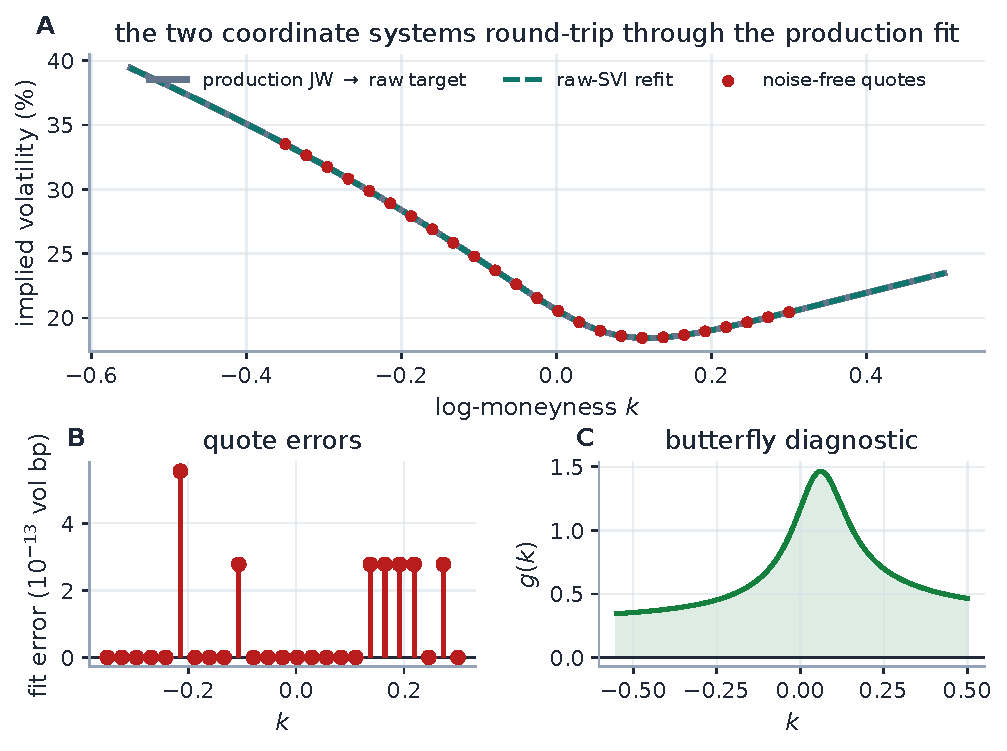
\includegraphics[width=\textwidth]{fig_svimom_recovery.pdf}
\caption{The two coordinate systems round-trip through the production fit.
Panel A: target and refit coincide, so the useful evidence is the residual scale
(Panel B, in $10^{-13}$ vol bp) and the independent Durrleman diagnostic
(Panel C).  The test exercises conversion, initialization, calibration and
reverse readout in one reproducible path; it deliberately says nothing about
real-market fit.}
\label{fig:recovery}
\end{figure}

\begin{heuristic}
On real NBBO history the published spike-regime replay measured SVI at
\svimomhistin\ vol bp RMS in-sample and \svimomhistoos\ out-of-sample across
$\approx\svimomnodes$ nodes per regime --- an order of magnitude worse than the
laboratory number above, and the honest figure of merit.  SVI is also stiffer
than LQD or Local-Vol on event or double-hump shapes, for the reason
\cref{sec:rigidity} makes precise.  (Those replay parquets are historical and
not checked into this workspace; the numbers are retained for continuity with
the note and deck.)
\end{heuristic}

%======================================================================
\section{One belly, one turn}
\label{sec:rigidity}

Strict convexity, $w''>0$, buys SVI one minimum and one monotone turn of the
slope from $-\betL$ to $+\betR$.  On a liquid equity-index chain this is exactly
the right regularization: it forbids the wiggles that noise would otherwise
carve into a smile.  But it is also a hard expressiveness ceiling.  A W-shaped
total-variance target (Note~03), a double-humped event density (Note~01's
double-hat), or a sharply localized short-dated kink asks the curve to turn more
than once, and one hyperbola has exactly one belly.  \Cref{fig:rigidity} makes
the failure quantitative: against a smooth, positive, deliberately two-minimum
target, production raw SVI returns the best single-belly compromise, missing by
\svimomrigidrms\ vol bp RMS and \svimomrigidmax\ vol bp at worst.

\begin{figure}[H]
\centering
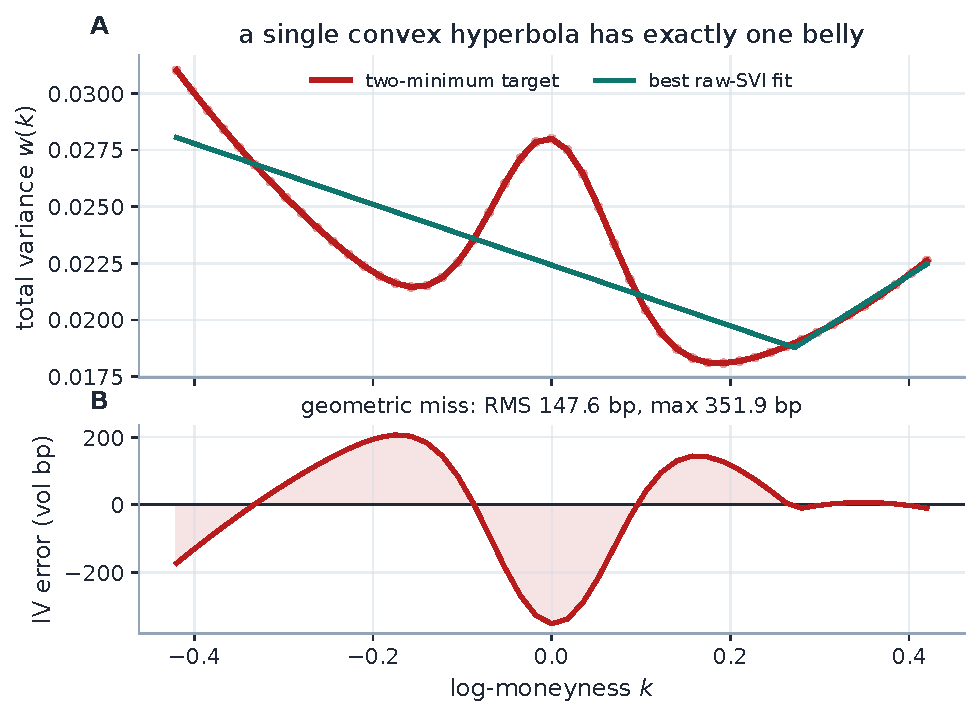
\includegraphics[width=0.96\textwidth]{fig_svimom_rigidity.pdf}
\caption{A geometric stress test, not a market smile.  The synthetic target has
two minima and a central hump; one convex hyperbola cannot follow it and settles
for the best compromise (A), leaving the structured residual of Panel B.  This
is the price of the convexity that regularizes ordinary smiles.}
\label{fig:rigidity}
\end{figure}

Sparse identification is a second, subtler limitation, and it is where the
tail/belly reading pays off once more.  On a narrow or one-sided quote window
the initializer's ``wing slopes'' are finite-span proxies read off the quoted
range, not asymptotic observations, and distinct raw tuples can price the quoted
strikes almost identically while implying different remote wings.  The fitted
\emph{curve} can be stable even when $(a,b,\rho,m,s)$ is not.  JW is easier to
read, but its tail handles $p,c$ are still \emph{extrapolated} functionals when
the market has not quoted the wings.  Across fits, compare prices, curves, and
observed handles --- not raw coefficients.

\paragraph{Exercise 3.}
The two-minimum target of \cref{fig:rigidity} is positive and smooth but not
convex.  Argue directly from $w''>0$ that no raw SVI slice can have two local
minima, and hence that the RMS miss cannot be driven to zero by any choice of
$(a,b,\rho,m,s)$ --- the limitation is structural, not a matter of optimizer
tuning.

%======================================================================
\section{What is genuinely original, and limitations}
\label{sec:original}

SVI, the jump-wing handles, and the arbitrage analysis are classical: raw SVI
and JW are due to Gatheral, the arbitrage-free theory to Gatheral--Jacquier and
Durrleman, the wing bound to Lee, and the exact butterfly domain to
Martini--Mingone.  The reading offered here --- \emph{wings as a moment reading
of the tails, belly as the interior the cheap screens cannot reach} --- is a
framing, not a theorem.  The implementation choices worth flagging are three:
\emph{structural validity by reparametrization} \eqref{eq:reparam}, so the solver
cannot leave tier one except through the two soft tail fences; the \emph{exact
raw$\leftrightarrow$JW conversion with a proved regular domain and an identified
belly blind spot} (\cref{thm:image}, \cref{rem:psi0}); and the \emph{analytic LM
Jacobian} that makes SVI the speed peer of the other overlays.

Limitations, stated plainly, because a lecture that sells a model without drawing
its boundary is an advertisement.  Raw SVI total variance is one globally convex
hyperbola with a single belly, so it cannot reproduce a W-shaped smile and can
over-smooth a sharp short-dated skew (\cref{sec:rigidity}).  It is
butterfly-clean only over a cone the coded fences do not certify
(\cref{sec:belly}), and carries no calendar coupling on its own --- that is
supplied, softly, by the model-agnostic hinge of Note~10.  On sparse or
one-sided chains its raw parameters can be poorly identified even where the
curve is stable, so comparisons should be made on curves and handles, never on
$(a,b,\rho,m,s)$.  And the jump-wing chart, elegant as it is, tears on the
$\psi=0$ stratum, where it keeps the tails and forgets the belly.

\appendix
%======================================================================
\section{Hyperparameter atlas}
\label{app:atlas}

\begin{longtable}{@{}p{0.25\textwidth}p{0.13\textwidth}p{0.54\textwidth}@{}}
\caption{SVI and shared calibration controls.}\label{tab:atlas}\\
\toprule Knob & Default & Role\\ \midrule
\endfirsthead
\toprule Knob & Default & Role\\ \midrule
\endhead
\multicolumn{3}{@{}l}{\emph{Surfaced (FitSettings / OptionsSettings)}}\\ \midrule
\texttt{model} & \texttt{lqd} & Set to \texttt{svi} to display the raw-SVI
overlay.\\
\texttt{sviPenaltyWeight} $W$ & \svimompenalty & Residual multiplier of the two
tail rows \eqref{eq:penalties} (effective $W^2$ in the squared cost; $0$ = fences
off).\\
\texttt{leeSlopeMax} $\beta_{\max}$ & \svimomleecap & Lee wing-slope cap on
$b(1+|\rho|)$; values $>2$ are accepted (a fence, not a guarantee).\\
\texttt{weightScheme} & \texttt{equal} & Per-quote weights, \texttt{equal} /
\texttt{tv\_density} (Note~07); arbitrary weights exist only at the low-level
API.\\
\texttt{midAnchorWeight} & $0.05$ & Mid anchor in the band-fit objective
(Note~07).\\
\texttt{haircut} & $0.005$ & Absolute-vol tightening, haircut band mode only.\\
\texttt{calendarWeight} & $10^{6}$ & Calendar hinge weight (Note~10; squared
objective, residual uses its root).\\
\texttt{extrapEnforce} & off & Tapered extrapolated-region fences
(\cref{sec:belly}); calibration-affecting, hybrid Jacobian when on.\\
\midrule
\multicolumn{3}{@{}l}{\emph{Internal (reparametrization / solver)}}\\ \midrule
$b=\operatorname{softplus}(\theta_2)$ & --- & Enforces $b>0$.\\
$\rho=\tanh(\theta_3)$ & --- & Enforces $|\rho|<1$.\\
$s=e^{\theta_5}$ & --- & Enforces $s>0$.\\
LM tolerances & $10^{-15}$ & \texttt{xtol/ftol/gtol}; LM converges in few
iterations, so tight tolerances are cheap.\\
trial-$w$ floor & $10^{-12}$ & Inside $\sqrt{w/\tau}$, to keep the IV residual
evaluable on structurally-valid-but-negative-variance trials; not part of
\texttt{RawSVI.implied\_vol}.\\
\bottomrule
\end{longtable}

%======================================================================
\section{Performance notes}
\label{app:perf}

\begin{enumerate}[leftmargin=1.6em]
\item \textbf{Levenberg--Marquardt over trust region.} On real noisy chains LM
crosses the penalty kinks in fewer iterations than \texttt{trf} at matched
tolerance; \texttt{trf} at $10^{-10}$ was measured slower on real nodes.
\item \textbf{Analytic Jacobian.} Closed-form Jacobian of the core residual
stack (data $+$ tail penalties $+$ calendar) through the reparametrization, with
the two scopes stated: the note's microbenchmark (25 synthetic quotes, core rows
only, single-threaded development machine, warmed median of five) measured
\svimomanalyticms\,ms vs \svimomfdms\,ms (\svimomspeedup$\times$) with objective
costs agreeing to \svimomcostdiff\ --- same solution within fit precision, not
bit-identical; the historical real-node measurement (spike-regime backtest
nodes, June-2026 harness) was \svimomhistbefore\,ms $\to$ \svimomhistafter\,ms
($\approx\svimomhistspeedup\times$).  Machine-dependent numbers belong here, not
in the body.  Gated to the var-swap/prior-free configuration; hybrid (analytic
core $+$ FD extrapolation rows) under \texttt{extrapEnforce}.
\item \textbf{Structural validity by construction.} The reparametrization
removes box-constraint handling, so each LM step is a plain linear solve.
\item \textbf{Geometric warm start.} Reading $(a,m)$ from the belly and
$(b,\rho)$ from the wing slopes lands $\theta_0$ close enough that liquid smiles
converge in a single pass.
\item \textbf{Converter conditioning.} The reference inverse of \cref{app:ref}
uses the cancellation-free denominator of \cref{rem:psi0}; it still rejects the
singular stratum, because no rearrangement can select a missing belly curvature.
\end{enumerate}

%======================================================================
\section{Traceability}
\label{app:trace}

A word on what these anchors prove, so they are not over-read.  The benchmark-fit
tests exercise an already tail-clean target, so the ``enforcement'' rows lock
that clean fits are untouched and that the penalty rows and their Jacobians are
correct when active --- they do not demonstrate that an adversarial fit ends
feasible.  The recovery test whose name says ``machine precision'' asserts
parameter agreement at $\sim10^{-4}$ relative and curve agreement at
$\sim10^{-6}$; the freshly generated example reaches machine precision, but the
lock is looser than its name.  A finite diagnostic grid is not a global proof.

\begingroup
\small
\setlength{\tabcolsep}{4pt}
\renewcommand{\arraystretch}{1.14}
\begin{longtable}{@{}p{0.32\textwidth}p{0.12\textwidth}p{0.50\textwidth}@{}}
\caption{Claims in this note and the code/tests that lock them.}\\
\toprule Claim & Object & Code anchor \newline \emph{Test anchors}\\ \midrule
\endfirsthead
\toprule Claim & Object & Code anchor \newline \emph{Test anchors}\\ \midrule
\endhead
Wing slopes are $b(1\mp\rho)$; tail limit of $g$ is $(4-\beta^2)/16$ &
\cref{prop:geom}, \cref{prop:tail} &
\nolinkurl{models/svi_jw/svi.py::RawSVI.wing_slopes}\newline
\nolinkurl{backtest/dispatch.py::_analytic_butterfly}\\
\addlinespace
JW$\to$raw conversion exact on the benchmark &
\cref{sec:jw} &
\nolinkurl{models/svi_jw/svi.py::jw_to_raw}\newline
\nolinkurl{test_lqd_pricing.py::test_jw_conversion_matches_note}\\
\addlinespace
Regular inverse domain; $\psi=0$ non-identification; invalid-input behaviour &
\cref{thm:image}, \cref{rem:psi0} &
\nolinkurl{models/svi_jw/svi.py}\newline
\nolinkurl{test_svi_domain.py::test_regular_domain_round_trips}\newline
\nolinkurl{::test_psi_zero_stratum_not_identified}\newline
\nolinkurl{::test_invalid_inputs_fail_loudly_not_plausibly}\\
\addlinespace
Tail screens do not certify butterfly freedom (Axel Vogt slice) &
\cref{sec:belly} &
\nolinkurl{models/svi_jw/calibrate.py::_penalties}\newline
\nolinkurl{test_svi_domain.py::test_core_screens_do_not_certify_butterfly_freedom}\\
\addlinespace
Noise-free benchmark recovery (params $\sim10^{-4}$ rel, curve $\sim10^{-6}$) &
\cref{sec:example} &
\nolinkurl{models/svi_jw/calibrate.py}\newline
\nolinkurl{test_svi_calibrate.py::test_recovers_benchmark_parameters}\newline
\nolinkurl{::test_curve_reproduced_to_machine_precision} (name predates the
looser lock)\\
\addlinespace
Clean fits untouched by the fences (benchmark is tail-clean) &
\cref{prop:screensjw} &
\nolinkurl{models/svi_jw/calibrate.py::_penalties}\newline
\nolinkurl{test_svi_calibrate.py::test_respects_lee_wing_bound}\newline
\nolinkurl{::test_min_variance_non_negative}\\
\addlinespace
Analytic Jacobian matches FD, penalty rows active or not &
\cref{sec:jacobian} &
\nolinkurl{models/svi_jw/jacobian.py}\newline
\nolinkurl{test_svi_jacobian.py::test_mid_fit_admissible}\newline
\nolinkurl{::test_lee_penalty_active}\newline
\nolinkurl{::test_min_variance_penalty_active}\\
\addlinespace
Calendar hinge rows correct; off is byte-identical &
\cref{sec:calib} &
\nolinkurl{models/svi_jw/calibrate.py}\newline
\nolinkurl{test_svi_jacobian.py::test_calendar_floor_active}\newline
\nolinkurl{test_overlay_calendar.py::test_svi_no_floor_is_byte_identical}\\
\addlinespace
Prior blocks reach the SVI overlay &
\cref{sec:calib} &
\nolinkurl{models/svi_jw/calibrate.py}\newline
\nolinkurl{test_prior_parametric.py::test_operator_prior_pulls_all_models_toward_prior_skew}\\
\bottomrule
\end{longtable}
\endgroup

%======================================================================
\section{Reference implementation: the two maps}
\label{app:ref}

The raw slice evaluates in one line, $w(k)=a+b(\rho(k-m)+\sqrt{(k-m)^2+s^2})$;
the maps below read the handles off it and invert them.  The listing is imported
and executed by \texttt{figures/gen\_svi\_moments.py}, which compares the checked
inverse against production \texttt{jw\_to\_raw} on three regular-domain points to
relative tolerance $2\times10^{-12}$ before any figure is written --- so the code
printed here is the code that produced the note's numbers.  The inverse uses the
cancellation-free denominator of \cref{rem:psi0}; the reverse map is exactly the
functional definition \eqref{eq:rawtojw}.

\lstinputlisting[caption={Executable raw/JW reference maps used by this note
(\texttt{figures/svi\_moments\_reference.py}).},label={lst:ref}]%
{figures/svi_moments_reference.py}

\begin{thebibliography}{9}
\bibitem{Gatheral2004} J.~Gatheral. A parsimonious arbitrage-free implied
volatility parameterization with application to the valuation of volatility
derivatives. Presentation, Global Derivatives, Madrid, 2004.
\bibitem{GatheralJacquier2014} J.~Gatheral and A.~Jacquier. Arbitrage-free SVI
volatility surfaces. \emph{Quantitative Finance}, 14(1):59--71, 2014.
\bibitem{Lee2004} R.~W.~Lee. The moment formula for implied volatility at
extreme strikes. \emph{Mathematical Finance}, 14(3):469--480, 2004.
\bibitem{Durrleman2010} V.~Durrleman. From implied to spot volatilities.
\emph{Finance and Stochastics}, 14(2):157--177, 2010.
\bibitem{MartiniMingone2022} C.~Martini and A.~Mingone. No arbitrage SVI.
\emph{SIAM Journal on Financial Mathematics}, 13(1):227--261, 2022.
\end{thebibliography}

\end{document}
